\documentclass[10pt,a4paper]{article}
\usepackage[T1]{fontenc}
\usepackage[utf8]{inputenc}
\usepackage{lmodern}
\usepackage[margin=2cm]{geometry}
\usepackage{amsmath,amssymb,amsthm}
\usepackage{booktabs,graphicx,xcolor,url}
\usepackage[hidelinks]{hyperref}
\newtheorem{proposition}{Proposition}
\newtheorem{fact}{Fact}
\newcommand{\symq}{\textsf{SymQ}}
\newcommand{\GF}{\mathrm{GF}(2)}
% Generated by paper/tools/make_tables.py from sealed results; do not edit.
\newif\ifblindrun
\blindrunfalse
\newcommand{\BOrderCells}{210}
\newcommand{\BOrderCircuits}{30}
\newcommand{\BOrderCommit}{e71c7e0fc8a2}
\newcommand{\BOrderCompared}{15}
\newcommand{\BOrderComplete}{15}
\newcommand{\BOrderDisagree}{0}
\newcommand{\BOrderIdBest}{0}
\newcommand{\BOrderIdTimeGeo}{3.56}
\newcommand{\BOrderIdTimeWorst}{164.4}
\newcommand{\BOrderIdTimeWorstCircuit}{adder\_16}
\newcommand{\BOrderNone}{11}
\newcommand{\BOrderOk}{124}
\newcommand{\BOrderRescued}{4}
\newcommand{\BOrderRescuedList}{\texttt{adder{\_}24}, \texttt{adder{\_}31}, \texttt{cadder{\_}24}, \texttt{cadder{\_}30}}
\newcommand{\BOrderSpreadGeo}{5.36}
\newcommand{\BOrderSpreadMax}{85}
\newcommand{\BOrderSpreadMaxCircuit}{adder\_16}
\newcommand{\NQCircuits}{19}
\newcommand{\QBDDEq}{2.62}
\newcommand{\QBDDEqHi}{3.17}
\newcommand{\QBDDEqLo}{2.16}
\newcommand{\QBDDEqMax}{5.47}
\newcommand{\QBDDEqMin}{0.99}
\newcommand{\QBDDEqN}{19}
\newcommand{\QBDDEqWarm}{2.58}
\newcommand{\QBDDEqWarmHi}{2.85}
\newcommand{\QBDDEqWarmLo}{2.37}
\newcommand{\QBDDEqWarmMax}{4.56}
\newcommand{\QBDDEqWarmMin}{2.13}
\newcommand{\QBDDEqWarmN}{19}
\newcommand{\QBDDEqWarmWins}{19}
\newcommand{\QBDDEqWins}{18}
\newcommand{\QBDDLoopCells}{57}
\newcommand{\QBDDLoopError}{0}
\newcommand{\QBDDLoopOk}{57}
\newcommand{\QBDDLoopSilent}{0}
\newcommand{\QBDDLoopUnfinished}{0}
\newcommand{\QBDDNeq}{3.33}
\newcommand{\QBDDNeqHi}{4.00}
\newcommand{\QBDDNeqLo}{2.77}
\newcommand{\QBDDNeqMax}{7.91}
\newcommand{\QBDDNeqMin}{1.59}
\newcommand{\QBDDNeqN}{19}
\newcommand{\QBDDNeqWarm}{2.63}
\newcommand{\QBDDNeqWarmHi}{3.03}
\newcommand{\QBDDNeqWarmLo}{2.35}
\newcommand{\QBDDNeqWarmMax}{7.15}
\newcommand{\QBDDNeqWarmMin}{2.07}
\newcommand{\QBDDNeqWarmN}{19}
\newcommand{\QBDDNeqWarmWins}{19}
\newcommand{\QBDDNeqWins}{19}
\newcommand{\QBDDSim}{3.86}
\newcommand{\QBDDSimHi}{5.18}
\newcommand{\QBDDSimLo}{3.08}
\newcommand{\QBDDSimMax}{32.16}
\newcommand{\QBDDSimMin}{1.92}
\newcommand{\QBDDSimN}{19}
\newcommand{\QBDDSimWarm}{2.46}
\newcommand{\QBDDSimWarmHi}{2.72}
\newcommand{\QBDDSimWarmLo}{2.27}
\newcommand{\QBDDSimWarmMax}{4.13}
\newcommand{\QBDDSimWarmMin}{2.01}
\newcommand{\QBDDSimWarmN}{19}
\newcommand{\QBDDSimWarmWins}{19}
\newcommand{\QBDDSimWins}{19}
\newcommand{\QBadWitness}{0}
\newcommand{\QCommit}{23469829a0dc}
\newcommand{\QCoreEq}{4.16}
\newcommand{\QCoreEqHi}{5.40}
\newcommand{\QCoreEqLo}{3.33}
\newcommand{\QCoreEqMax}{20.78}
\newcommand{\QCoreEqMin}{1.58}
\newcommand{\QCoreEqN}{19}
\newcommand{\QCoreEqWarm}{1.20}
\newcommand{\QCoreEqWarmHi}{1.23}
\newcommand{\QCoreEqWarmLo}{1.17}
\newcommand{\QCoreEqWarmMax}{1.39}
\newcommand{\QCoreEqWarmMin}{1.09}
\newcommand{\QCoreEqWarmN}{19}
\newcommand{\QCoreEqWarmWins}{19}
\newcommand{\QCoreEqWins}{19}
\newcommand{\QCoreNeq}{3.91}
\newcommand{\QCoreNeqHi}{4.76}
\newcommand{\QCoreNeqLo}{3.12}
\newcommand{\QCoreNeqMax}{8.74}
\newcommand{\QCoreNeqMin}{0.85}
\newcommand{\QCoreNeqN}{19}
\newcommand{\QCoreNeqWarm}{1.13}
\newcommand{\QCoreNeqWarmHi}{1.23}
\newcommand{\QCoreNeqWarmLo}{0.99}
\newcommand{\QCoreNeqWarmMax}{1.30}
\newcommand{\QCoreNeqWarmMin}{0.37}
\newcommand{\QCoreNeqWarmN}{19}
\newcommand{\QCoreNeqWarmWins}{18}
\newcommand{\QCoreNeqWins}{18}
\newcommand{\QCoreSim}{4.92}
\newcommand{\QCoreSimHi}{5.56}
\newcommand{\QCoreSimLo}{4.37}
\newcommand{\QCoreSimMax}{7.85}
\newcommand{\QCoreSimMin}{3.00}
\newcommand{\QCoreSimN}{19}
\newcommand{\QCoreSimWarm}{1.23}
\newcommand{\QCoreSimWarmHi}{1.25}
\newcommand{\QCoreSimWarmLo}{1.20}
\newcommand{\QCoreSimWarmMax}{1.34}
\newcommand{\QCoreSimWarmMin}{1.13}
\newcommand{\QCoreSimWarmN}{19}
\newcommand{\QCoreSimWarmWins}{19}
\newcommand{\QCoreSimWins}{19}
\newcommand{\QDisagree}{0}
\newcommand{\QDriverEq}{2.13}
\newcommand{\QDriverEqHi}{2.49}
\newcommand{\QDriverEqLo}{1.84}
\newcommand{\QDriverEqMax}{5.00}
\newcommand{\QDriverEqMin}{1.34}
\newcommand{\QDriverEqN}{19}
\newcommand{\QDriverEqWarm}{3.39}
\newcommand{\QDriverEqWarmHi}{3.52}
\newcommand{\QDriverEqWarmLo}{3.26}
\newcommand{\QDriverEqWarmMax}{3.85}
\newcommand{\QDriverEqWarmMin}{2.83}
\newcommand{\QDriverEqWarmN}{19}
\newcommand{\QDriverEqWarmWins}{19}
\newcommand{\QDriverEqWins}{19}
\newcommand{\QDriverNeq}{2.47}
\newcommand{\QDriverNeqHi}{3.01}
\newcommand{\QDriverNeqLo}{2.12}
\newcommand{\QDriverNeqMax}{10.54}
\newcommand{\QDriverNeqMin}{1.32}
\newcommand{\QDriverNeqN}{19}
\newcommand{\QDriverNeqWarm}{3.61}
\newcommand{\QDriverNeqWarmHi}{4.18}
\newcommand{\QDriverNeqWarmLo}{3.25}
\newcommand{\QDriverNeqWarmMax}{11.52}
\newcommand{\QDriverNeqWarmMin}{2.75}
\newcommand{\QDriverNeqWarmN}{19}
\newcommand{\QDriverNeqWarmWins}{19}
\newcommand{\QDriverNeqWins}{19}
\newcommand{\QDriverSim}{2.18}
\newcommand{\QDriverSimHi}{2.37}
\newcommand{\QDriverSimLo}{1.99}
\newcommand{\QDriverSimMax}{2.81}
\newcommand{\QDriverSimMin}{1.36}
\newcommand{\QDriverSimN}{19}
\newcommand{\QDriverSimWarm}{3.34}
\newcommand{\QDriverSimWarmHi}{3.53}
\newcommand{\QDriverSimWarmLo}{3.17}
\newcommand{\QDriverSimWarmMax}{3.98}
\newcommand{\QDriverSimWarmMin}{2.72}
\newcommand{\QDriverSimWarmN}{19}
\newcommand{\QDriverSimWarmWins}{19}
\newcommand{\QDriverSimWins}{19}
\newcommand{\QFusedVsLoopEq}{1.01}
\newcommand{\QFusedVsLoopEqHi}{1.07}
\newcommand{\QFusedVsLoopEqLo}{0.95}
\newcommand{\QFusedVsLoopEqN}{19}
\newcommand{\QFusedVsLoopEqWins}{10}
\newcommand{\QFusedVsLoopNeq}{1.01}
\newcommand{\QFusedVsLoopNeqHi}{1.09}
\newcommand{\QFusedVsLoopNeqLo}{0.93}
\newcommand{\QFusedVsLoopNeqN}{19}
\newcommand{\QFusedVsLoopNeqWins}{8}
\newcommand{\QFusedVsLoopSim}{0.97}
\newcommand{\QFusedVsLoopSimHi}{1.06}
\newcommand{\QFusedVsLoopSimLo}{0.89}
\newcommand{\QFusedVsLoopSimN}{19}
\newcommand{\QFusedVsLoopSimWins}{9}
\newcommand{\QFusionEq}{1.13}
\newcommand{\QFusionEqHi}{1.21}
\newcommand{\QFusionEqLo}{1.05}
\newcommand{\QFusionEqMax}{1.63}
\newcommand{\QFusionEqMin}{0.84}
\newcommand{\QFusionEqN}{19}
\newcommand{\QFusionEqWarm}{1.28}
\newcommand{\QFusionEqWarmHi}{1.44}
\newcommand{\QFusionEqWarmLo}{1.14}
\newcommand{\QFusionEqWarmMax}{1.99}
\newcommand{\QFusionEqWarmMin}{0.81}
\newcommand{\QFusionEqWarmN}{19}
\newcommand{\QFusionEqWarmWins}{16}
\newcommand{\QFusionEqWins}{17}
\newcommand{\QFusionNeq}{1.10}
\newcommand{\QFusionNeqHi}{1.19}
\newcommand{\QFusionNeqLo}{1.02}
\newcommand{\QFusionNeqMax}{1.50}
\newcommand{\QFusionNeqMin}{0.78}
\newcommand{\QFusionNeqN}{19}
\newcommand{\QFusionNeqWarm}{1.27}
\newcommand{\QFusionNeqWarmHi}{1.46}
\newcommand{\QFusionNeqWarmLo}{1.11}
\newcommand{\QFusionNeqWarmMax}{2.25}
\newcommand{\QFusionNeqWarmMin}{0.79}
\newcommand{\QFusionNeqWarmN}{19}
\newcommand{\QFusionNeqWarmWins}{16}
\newcommand{\QFusionNeqWins}{15}
\newcommand{\QFusionSim}{1.14}
\newcommand{\QFusionSimHi}{1.27}
\newcommand{\QFusionSimLo}{1.03}
\newcommand{\QFusionSimMax}{1.81}
\newcommand{\QFusionSimMin}{0.80}
\newcommand{\QFusionSimN}{19}
\newcommand{\QFusionSimWarm}{1.31}
\newcommand{\QFusionSimWarmHi}{1.54}
\newcommand{\QFusionSimWarmLo}{1.12}
\newcommand{\QFusionSimWarmMax}{2.62}
\newcommand{\QFusionSimWarmMin}{0.77}
\newcommand{\QFusionSimWarmN}{19}
\newcommand{\QFusionSimWarmWins}{14}
\newcommand{\QFusionSimWins}{13}
\newcommand{\QGroups}{57}
\newcommand{\QMaxTerms}{8\,520}
\newcommand{\QNativeEqMedianMs}{0.10}
\newcommand{\QNativeFusedCells}{57}
\newcommand{\QNativeFusedError}{0}
\newcommand{\QNativeFusedOk}{57}
\newcommand{\QNativeFusedSilent}{0}
\newcommand{\QNativeFusedUnfinished}{0}
\newcommand{\QNativeLoopCells}{57}
\newcommand{\QNativeLoopError}{0}
\newcommand{\QNativeLoopOk}{57}
\newcommand{\QNativeLoopSilent}{0}
\newcommand{\QNativeLoopUnfinished}{0}
\newcommand{\QOrderCells}{133}
\newcommand{\QOrderCircuits}{19}
\newcommand{\QOrderCommit}{e71c7e0fc8a2}
\newcommand{\QOrderCompared}{19}
\newcommand{\QOrderComplete}{19}
\newcommand{\QOrderDisagree}{0}
\newcommand{\QOrderIdBest}{6}
\newcommand{\QOrderIdTimeGeo}{1.26}
\newcommand{\QOrderIdTimeWorst}{5.1}
\newcommand{\QOrderIdTimeWorstCircuit}{c2\_181}
\newcommand{\QOrderNone}{0}
\newcommand{\QOrderOk}{133}
\newcommand{\QOrderRescued}{0}
\newcommand{\QOrderRescuedList}{none}
\newcommand{\QOrderSpreadGeo}{1.79}
\newcommand{\QOrderSpreadMax}{146}
\newcommand{\QOrderSpreadMaxCircuit}{c2\_181}
\newcommand{\QPBEq}{2.98}
\newcommand{\QPBEqHi}{3.42}
\newcommand{\QPBEqLo}{2.59}
\newcommand{\QPBEqMax}{4.70}
\newcommand{\QPBEqMin}{1.76}
\newcommand{\QPBEqN}{19}
\newcommand{\QPBEqWarm}{2.12}
\newcommand{\QPBEqWarmHi}{2.18}
\newcommand{\QPBEqWarmLo}{2.05}
\newcommand{\QPBEqWarmMax}{2.39}
\newcommand{\QPBEqWarmMin}{1.84}
\newcommand{\QPBEqWarmN}{19}
\newcommand{\QPBEqWarmWins}{19}
\newcommand{\QPBEqWins}{19}
\newcommand{\QPBFusedEq}{2.98}
\newcommand{\QPBFusedEqHi}{3.36}
\newcommand{\QPBFusedEqLo}{2.59}
\newcommand{\QPBFusedEqMax}{4.19}
\newcommand{\QPBFusedEqMin}{1.53}
\newcommand{\QPBFusedEqN}{19}
\newcommand{\QPBFusedEqWarm}{2.23}
\newcommand{\QPBFusedEqWarmHi}{2.54}
\newcommand{\QPBFusedEqWarmLo}{1.95}
\newcommand{\QPBFusedEqWarmMax}{3.61}
\newcommand{\QPBFusedEqWarmMin}{1.32}
\newcommand{\QPBFusedEqWarmN}{19}
\newcommand{\QPBFusedEqWarmWins}{19}
\newcommand{\QPBFusedEqWins}{19}
\newcommand{\QPBFusedNeq}{3.31}
\newcommand{\QPBFusedNeqHi}{3.50}
\newcommand{\QPBFusedNeqLo}{3.12}
\newcommand{\QPBFusedNeqMax}{4.23}
\newcommand{\QPBFusedNeqMin}{2.64}
\newcommand{\QPBFusedNeqN}{19}
\newcommand{\QPBFusedNeqWarm}{2.22}
\newcommand{\QPBFusedNeqWarmHi}{2.61}
\newcommand{\QPBFusedNeqWarmLo}{1.89}
\newcommand{\QPBFusedNeqWarmMax}{4.08}
\newcommand{\QPBFusedNeqWarmMin}{1.30}
\newcommand{\QPBFusedNeqWarmN}{19}
\newcommand{\QPBFusedNeqWarmWins}{19}
\newcommand{\QPBFusedNeqWins}{19}
\newcommand{\QPBFusedSim}{4.01}
\newcommand{\QPBFusedSimHi}{4.37}
\newcommand{\QPBFusedSimLo}{3.67}
\newcommand{\QPBFusedSimMax}{6.00}
\newcommand{\QPBFusedSimMin}{2.85}
\newcommand{\QPBFusedSimN}{19}
\newcommand{\QPBFusedSimWarm}{2.14}
\newcommand{\QPBFusedSimWarmHi}{2.52}
\newcommand{\QPBFusedSimWarmLo}{1.83}
\newcommand{\QPBFusedSimWarmMax}{3.86}
\newcommand{\QPBFusedSimWarmMin}{1.22}
\newcommand{\QPBFusedSimWarmN}{19}
\newcommand{\QPBFusedSimWarmWins}{19}
\newcommand{\QPBFusedSimWins}{19}
\newcommand{\QPBLoopCells}{57}
\newcommand{\QPBLoopError}{0}
\newcommand{\QPBLoopOk}{57}
\newcommand{\QPBLoopSilent}{0}
\newcommand{\QPBLoopUnfinished}{0}
\newcommand{\QPBNeq}{3.28}
\newcommand{\QPBNeqHi}{3.61}
\newcommand{\QPBNeqLo}{2.97}
\newcommand{\QPBNeqMax}{4.54}
\newcommand{\QPBNeqMin}{2.21}
\newcommand{\QPBNeqN}{19}
\newcommand{\QPBNeqWarm}{2.15}
\newcommand{\QPBNeqWarmHi}{2.24}
\newcommand{\QPBNeqWarmLo}{2.07}
\newcommand{\QPBNeqWarmMax}{2.42}
\newcommand{\QPBNeqWarmMin}{1.80}
\newcommand{\QPBNeqWarmN}{19}
\newcommand{\QPBNeqWarmWins}{19}
\newcommand{\QPBNeqWins}{19}
\newcommand{\QPBSim}{4.16}
\newcommand{\QPBSimHi}{4.67}
\newcommand{\QPBSimLo}{3.68}
\newcommand{\QPBSimMax}{5.92}
\newcommand{\QPBSimMin}{2.22}
\newcommand{\QPBSimN}{19}
\newcommand{\QPBSimWarm}{2.11}
\newcommand{\QPBSimWarmHi}{2.19}
\newcommand{\QPBSimWarmLo}{2.03}
\newcommand{\QPBSimWarmMax}{2.37}
\newcommand{\QPBSimWarmMin}{1.79}
\newcommand{\QPBSimWarmN}{19}
\newcommand{\QPBSimWarmWins}{19}
\newcommand{\QPBSimWins}{19}
\newcommand{\QQCECCells}{57}
\newcommand{\QQCECEq}{32.50}
\newcommand{\QQCECEqHi}{50.63}
\newcommand{\QQCECEqLo}{21.34}
\newcommand{\QQCECEqMax}{422.77}
\newcommand{\QQCECEqMin}{7.43}
\newcommand{\QQCECEqN}{19}
\newcommand{\QQCECEqWins}{19}
\newcommand{\QQCECError}{0}
\newcommand{\QQCECMinMs}{1.7}
\newcommand{\QQCECNeq}{38.35}
\newcommand{\QQCECNeqHi}{51.06}
\newcommand{\QQCECNeqLo}{27.49}
\newcommand{\QQCECNeqMax}{97.81}
\newcommand{\QQCECNeqMin}{5.72}
\newcommand{\QQCECNeqN}{19}
\newcommand{\QQCECNeqWins}{19}
\newcommand{\QQCECOk}{38}
\newcommand{\QQCECSilent}{0}
\newcommand{\QQCECUnfinished}{0}
\newcommand{\QSortingEq}{0.89}
\newcommand{\QSortingEqHi}{0.95}
\newcommand{\QSortingEqLo}{0.83}
\newcommand{\QSortingEqMax}{1.25}
\newcommand{\QSortingEqMin}{0.55}
\newcommand{\QSortingEqN}{19}
\newcommand{\QSortingEqWarm}{0.82}
\newcommand{\QSortingEqWarmHi}{0.83}
\newcommand{\QSortingEqWarmLo}{0.81}
\newcommand{\QSortingEqWarmMax}{0.86}
\newcommand{\QSortingEqWarmMin}{0.77}
\newcommand{\QSortingEqWarmN}{19}
\newcommand{\QSortingEqWarmWins}{0}
\newcommand{\QSortingEqWins}{2}
\newcommand{\QSortingNeq}{0.91}
\newcommand{\QSortingNeqHi}{0.95}
\newcommand{\QSortingNeqLo}{0.88}
\newcommand{\QSortingNeqMax}{1.14}
\newcommand{\QSortingNeqMin}{0.79}
\newcommand{\QSortingNeqN}{19}
\newcommand{\QSortingNeqWarm}{0.81}
\newcommand{\QSortingNeqWarmHi}{0.82}
\newcommand{\QSortingNeqWarmLo}{0.80}
\newcommand{\QSortingNeqWarmMax}{0.86}
\newcommand{\QSortingNeqWarmMin}{0.71}
\newcommand{\QSortingNeqWarmN}{19}
\newcommand{\QSortingNeqWarmWins}{0}
\newcommand{\QSortingNeqWins}{3}
\newcommand{\QSortingSim}{0.85}
\newcommand{\QSortingSimHi}{0.90}
\newcommand{\QSortingSimLo}{0.81}
\newcommand{\QSortingSimMax}{1.00}
\newcommand{\QSortingSimMin}{0.65}
\newcommand{\QSortingSimN}{19}
\newcommand{\QSortingSimWarm}{0.78}
\newcommand{\QSortingSimWarmHi}{0.82}
\newcommand{\QSortingSimWarmLo}{0.73}
\newcommand{\QSortingSimWarmMax}{0.88}
\newcommand{\QSortingSimWarmMin}{0.55}
\newcommand{\QSortingSimWarmN}{19}
\newcommand{\QSortingSimWarmWins}{0}
\newcommand{\QSortingSimWins}{0}
\newcommand{\QWrong}{0}
\newcommand{\SetupBDD}{2.659}
\newcommand{\SetupNative}{0.010}
\newcommand{\SetupPB}{4.108}

\newcommand{\QualTrials}{4320}
\newcommand{\QualCases}{8}
\newcommand{\QualFamilies}{4}
\newcommand{\QualRunTrials}{2700}
\newcommand{\QualRunCases}{5}
\newcommand{\QualRunFamilies}{4}
\newcommand{\QualMaxTerms}{200000}
\newcommand{\QualMaxNodes}{1000000}
\newcommand{\QualCommit}{\texttt{49f5c438fe8916d2d2abf0a1dd137c33fd752184}}
\newcommand{\QualNative}{\texttt{2a14a3eac241d2e4de22ebda12880505f8bf0b63b4d07f6a9c9460269b4a8bc4}}
\newcommand{\QualRawHash}{\texttt{20810d3735be03677f5245f695dd01683d483b6be8b0494ec6d42615a2d95573}}
\newcommand{\QualArtifactHash}{\texttt{797e79198d67d5a6af5fa66b822d1e6936281765bf5916488763f302b6f298c2}}
\newcommand{\QualClassificationHash}{\texttt{2604175d57a3100d420cce3826a6ffdaa850ffa1593d017db27c37a8d9e2b242}}

\title{SymQ: Exact ANF Inspection and Equivalence Checking\\
for Reversible Boolean Circuits\\
\large Task-separated qualification of a specialized native engine}
\author{Joshua Melka\\\small Independent researcher (no affiliation)}
\date{Research revision, 30 October 2026 --- not submitted}
\begin{document}
\maketitle

\begin{abstract}
We study an engineering trade-off in compiler verification: obtaining exact Boolean output
functions and replayable counterexamples can cost more than deciding equivalence alone.
SymQ represents algebraic normal forms (ANFs) as monomial zero-suppressed decision diagrams,
a representation established by PolyBoRi and earlier functional-diagram work. Its contribution
is a specialized budgeted implementation and inspectable experimental evidence, rather than
a new algebraic algorithm. We separate simulation, explicit ANF materialization, equivalence,
counterexample production and full benchmark service-call cost; SAT and quantum decision procedures are
compared only where their semantic service matches. A source- and binary-pinned short
qualification records \QualTrials{} planned trials over \QualCases{} cases in
\QualFamilies{} families; \QualRunTrials{} trials on \QualRunCases{} cases in
\QualRunFamilies{} families were attempted, with failures, unsupported requests and unrun
cases retained. It validates
a protocol on that bounded corpus, not broad competitiveness. Earlier measurements are
preserved as historical, including adverse families, resource failures and corrected timing
boundaries; they are not relabeled as current results. Monomial expansion and variable order
remain important limitations. We claim neither a new representation, universal speedup,
independently certified equivalence nor general quantum-program verification.
\end{abstract}

\section{A compiler-facing question and contribution}
Reversible X, CX, CCX and MCX circuits occur in arithmetic, oracles and
uncomputation~\cite{wille2008revlib,gidney2018halving}. Two equal-width programs in this
fragment compute permutations of the Boolean cube, so their full-input equivalence is a
classical functional question. A compiler may ask only whether a rewrite preserves that
function, or may also need explicit intermediate ANFs, dependency inspection and a sparse
counterexample. These services have different costs.

Our testable claim is narrow: a specialized native monomial-ZDD implementation can share
exact symbolic Boolean functions and replay distinguishing inputs, while its practical
position relative to explicit ANF, BDDs, PolyBoRi and SAT depends on the requested service,
family, order and budget. We supply (i) an explicit semantic contract and short derivations,
(ii) task-separated source-pinned qualification with raw status denominators, and
(iii) preserved historical evidence, including unfavorable results. These are implementation
and measurement contributions. The research implementation is not formally verified.

The historical paper branch used an older native binary and an explored corpus formerly
called blind. Current code has ABI-5 validation, bounded caches and explicit wider modes;
old timings cannot validate those changes. We therefore distinguish current qualification
from historical exploration throughout. A short successful run can qualify a harness and
its tested cases; it cannot establish machine-independent or cross-family superiority.

\section{Known foundations and relevant competitors}
Boolean ANFs are canonical square-free polynomial expansions. ZDDs~\cite{minato1993zdd,
minato1995polynomials,minato2001zdd} compactly represent set families; monomial families with
recursive Boolean-ring operations are central to PolyBoRi/BRiAl~\cite{brickenstein2009polybori,
brickenstein2008groebner,brial}. Positive-Davio functional diagrams describe the same
expansion under a fixed order~\cite{kebschull1992fdd,drechsler1996ofdd}. We claim no first
representation, multiplication recurrence or Boolean verification theorem.

CUDD BDDs~\cite{bryant1986graph,somenzi2015cudd,dd060} represent functions without expanding
ANF; their service may therefore be preferable for a verdict. DD and SAT checking of
reversible circuits already appear in Wille et al.~\cite{wille2009equivalence}. ABC combines
AIG techniques with SAT-based combinational equivalence~\cite{brayton2010abc,
mishchenko2006cec}. A PySAT miter, when measured, is a SAT baseline rather than a claim to
implement ABC. A solver need not export monomials to decide the same Boolean miter.

MQT QCEC~\cite{burgholzer2021advanced,burgholzer2021qcec,qcecrepo} can establish unitary
relations on a broader grammar. On the common reversible fragment, permutation-matrix
equality agrees with full functional equality, but QCEC supplies no output ANFs. Its phase
convention and enabled complete checkers must be recorded; inconclusive outcomes are not
differences. Path sums~\cite{amy2019towards}, QuPRS~\cite{huang2026quprs} and hybrid
methods address broader problems. Irene preserves factored XOR--AND graphs and reasons
with hybrid path sums and observable density kernels~\cite{ke2026irene}; phased
outcome-complete simulation tracks phases under declared rotation/outcome
correspondences~\cite{kliuchnikov2026phased}; deferred-measurement techniques lift unitary
checking to hybrid programs~\cite{ricciardi2025hybrid}. They are important prior art, not
unmatched speed comparisons. \path{paper/RELATED_WORK.md} records primary-source checks and
remaining search limitations.

\section{Contract and derivations}\label{sec:semantics}
A well-formed width-$n$ circuit is a finite sequence $(C,t)$ with distinct controls
$C\subseteq\{0,\ldots,n-1\}$ and $t\notin C$. Its gate updates
$s_t\leftarrow s_t\oplus\prod_{c\in C}s_c$, leaving other wires fixed; the empty product
is one. All $n$ inputs are independent and all outputs are compared in the declared order.
No clean ancilla, discarded output or legal-input predicate is inferred from circuit names.

Let $B_n=\GF[x_0,\ldots,x_{n-1}]/(x_i^2-x_i)$. Its unique ANF consists of distinct
square-free monomials; evaluation is a ring homomorphism to $\GF$ and identifies $B_n$
with Boolean functions. Symbolic simulation starts at $f_i=x_i$ and updates
$f_t\leftarrow f_t+\prod_{c\in C}f_c$.

\begin{proposition}[Classical correctness, standard]
For every input $a$, evaluating the symbolic outputs gives the concrete circuit output.
Consequently, equal-width circuits are functionally equivalent exactly when all output
ANFs agree.
\end{proposition}
\begin{proof}
Induct over gates. Initially $f_i(a)=a_i$. Evaluation preserves addition and multiplication,
so the symbolic target update evaluates to precisely the concrete XOR/product update.
Uniqueness of ANF then gives both directions of the equivalence criterion.
\end{proof}

\begin{proposition}[Minimum-degree distinguishing input]
If nonzero $p\in B_n$ contains a monomial $M$ of minimum cardinality, the assignment
$\chi_M$ with ones exactly on $M$ satisfies $p(\chi_M)=1$.
\end{proposition}
\begin{proof}
The evaluation counts modulo two the monomials of $p$ contained in $M$. A proper subset
would have smaller degree and cannot occur, so exactly $M$ contributes. The argument also
covers the constant monomial $M=\emptyset$.
\end{proof}
Applied to a differing output, this gives a concrete counterexample. Both circuits are
re-executed before accepting it. That replay validates a difference; it does not certify
an equivalence verdict or independently verify the implementation.

Fix a variable order. A ZDD node denotes $P_0+vP_1$, with ordered children, nonzero high child
and unique hash-consed triples. Root identity denotes equality only within the same manager
and generation. Cross-manager identifiers must never be compared directly. For
$P=P_0+vP_1$ and $Q=Q_0+vQ_1$,
\begin{equation}\label{eq:product}
PQ=P_0Q_0+v(P_0Q_1+P_1Q_0+P_1Q_1).
\end{equation}
Expansion and $v^2=v$ prove this familiar recursion. The alternative form is
$P_0Q_0+v((P_0+P_1)(Q_0+Q_1)+P_0Q_0)$; its low term is essential. No asymptotic advantage
is asserted for either form.

Budgets may abort but may not approximate. Under exact transitions, a completed in-budget
run has the unbudgeted semantics; a late or aborted run establishes neither equality nor
difference. This abstract observation does not prove responsiveness, safe cache recovery
or C memory correctness. Those require separate implementation invariants and tests.
The full model in \path{paper/FORMAL_MODEL.md} states manager ownership, root preservation,
resource and recovery hypotheses explicitly. None of these proofs is machine-checked.

\section{Implementation and task boundaries}\label{sec:implementation}
The current native implementation retains the ordinary 64-variable engine and an explicit
128-variable engine, with multiword import/export and high-bit witnesses. Width extension
changes admissibility, not exponential worst-case representation growth. Root sharing,
batched gate propagation and owned DAG transfer are engineering mechanisms, not new
mathematical decision procedures. Caches, live roots and temporary transfer peaks consume
resources even when the final function is small. No backend is silently selected to rescue
a failed declared engine. The primary \texttt{zdd-native-fused} configuration uses the
shipped public native gate loop; the secondary \texttt{zdd-native} benchmark configuration
explicitly substitutes a matched Python algebra loop. It is not the ordinary default, and
the two configurations must not be selected post hoc or pooled.

\begin{table}[tbp]
\centering\small
\caption{Services and comparison boundaries. Conversion and replay are included in the full benchmark
service cost when required. Actual public API calls, manual benchmark services and
conversion-excluded services retain distinct raw labels; no service is called kernel-only.}
\label{tab:services}
\begin{tabular}{p{2.5cm}p{5.4cm}p{7.0cm}}
\toprule
service & required output & eligible comparison \\
\midrule
Simulation & exact symbolic Boolean functions & ring/BDD engines; no monomial enumeration required \\
ANF export & explicit ANF of every retained wire & ring engines and a separately timed BDD-to-ANF conversion \\
Equivalence & exact full-input Boolean decision & symbolic engines, checked SAT miter; QCEC on common unitary grammar \\
Counterexample & distinguishing assignment, concretely replayed & only adapters actually returning a witness; verdict-only negatives do not qualify \\
\bottomrule
\end{tabular}
\end{table}

A native benchmark first validates the actual ABI, result shape, root count, loaded extension
and source and build fingerprints. Replacing an obsolete ABI assertion alone would not establish
compatibility. The harness exercises simulation and both verdict directions against an
independent small reference. No ABI-4 fallback or stale binary is retained to make tests pass.

\section{Current short qualification protocol}\label{sec:method}
The campaign is frozen before execution by its manifest, source commit, per-file hashes,
native binary hash and environment. Repetition order is randomized in paired blocks;
workers are fresh and resource-limited, with CPU, wall and memory boundaries recorded.
Teardown contributes to whole-worker lifetime; an exclusive cleanup duration is not
instrumented. The preregistered study combines newly seeded synthetic cases with a
deterministic increment calibration; it is not an entirely untouched holdout.
Whole-worker wall time extends through process reaping. Raw \texttt{cpu\_seconds}
is cumulative CPU sampled before result JSON encoding and teardown; those final CPU
costs are unmeasured. \texttt{service\_cpu\_seconds} runs through the service checkpoint,
including input materialization and orchestration, and therefore has a broader boundary
than the selected public-call \texttt{service\_seconds}. Validation CPU is separate.
Workers eagerly import the same optional-tool prefix before their service-ready checkpoint.
Its startup cost and memory remain in whole-worker measurements, outside service time.
Consequently, RSS here characterizes this qualification process envelope, not the memory
of a minimal deployment importing only its chosen backend or an isolated native heap.
The executed qualification subset is now explored; reserved unrun cases remain unmeasured,
not independently gathered external workloads. During execution, code inspection found that
the increment generator ignores its seed and its small-width instance had already been
used in development tests. Its raw \texttt{new\_holdout} label is therefore incorrect:
an adjudication sidecar classifies it as calibration while preserving the measured source,
manifest and raw bytes. No case was replaced or rerun. The original aggregate remains a
descriptive mixed-study result; a separately labeled post-audit holdout-only sensitivity
excludes calibration, leaving only two small oracle-eligible families. Its provenance
is synthetic unless a row identifies a pinned external generator and license; a fresh seed
is not evidence of external-workload generality.

The affine pair uses a random CNOT stream and independent Gaussian synthesis.
The triangular shear keeps its control wires fixed and compares ANF coefficients with
a truth-table-minterm implementation on the last target. Increment compares a carry
construction with complement/decrement/complement. The adverse nonlinear pairs instead
copy one random MCX stream and insert an adjacent cancelling CX pair into the candidate.
They stress propagation through a connected synthetic circuit; they are not independent
compiler outputs, and structural cancellation can avoid the symbolic work entirely.

The raw label \texttt{public\_api\_end\_to\_end} denotes the actual public API path named
in the artifact, loaded from the immutable source snapshot with dependencies installed in
the recorded environment. This is a source-snapshot performance campaign, not a wheel
performance campaign; independent wheel CI checks packaging separately. The frozen
manifest's older word ``installed'' does not change this loading boundary.
An inclusive API stage has no invented internal decomposition. The separate
\texttt{task\_service\_end\_to\_end} label denotes the manual benchmark pipeline with
input materialization, engine setup and required conversion/replay. A
\texttt{precompiled\_service} row excludes conversion but still includes setup; it is not
a kernel-only time. Independent oracle validation is separately timed outside service cost
under its own validation wall/CPU budget, within the complete worker envelope. The service
checkpoint survives optional validation failure: a fast completed service is not relabeled
a service timeout because its independent oracle later exhausts resources. Qualified
success, service completion and oracle/replay evidence therefore have distinct counts.

The raw artifact retains all requested trials: success, unsupported, not run, timeout, OOM,
inconclusive and error. A larger unrun instance is not counted as a measured timeout.
Computation, comparison, witness extraction/replay, export and validation have separate stage
fields; unavailable stages remain unavailable. A completed simulation is not automatically
a completed export. Likewise, a fingerprint singleton supplies no cross-backend agreement.
The declared analysis plan fixes the shipped fused native configuration as primary and
retains the matched Python-loop native configuration as a separate ablation.
Small all-input oracles and concretely checked mutants are correctness evidence distinct
from timing and from solver decisions.

Current conditional speed compares paired successful trials with independent small-domain
oracle checks for the same case, task and boundary. Larger cross-algorithm agreements are
separate evidence and do not silently acquire exhaustive-oracle status.
We take a median of paired ratios within each case, then give each case within a family and
each represented family equal weight. Descriptive resampling intervals and leave-one-family-out
sensitivity expose dependence and influence; a few synthetic families are not thirty
independent observations. No population-level generalization follows from this small set.
Coverage is separately reported under the joint declared policy: common process wall,
CPU and memory limits plus backend-specific cooperative representation guards.
The term threshold is \QualMaxTerms{} and the node threshold \QualMaxNodes{}, but these
are not equal abstract-work budgets. Sparse ANF checks explicit term counts and an
input-product-size bound; PolyBoRi checks polynomial term counts. Python/native ZDDs
limit retained manager nodes, while their compact functions need not satisfy the term
threshold until ANF materialization. CUDD limits manager nodes and applies the term
guard during conversion to ANF. SAT and QCEC receive their applicable timeout/process
limits, without artificial ANF-term or DD-node caps. Thus coverage is not a comparison
under CPU/RSS limits alone, and an early representation-guard refusal must not be
interpreted as exhaustion of a uniform amount of work.
Parent resource polling occurs at 10\,ms intervals; process termination and cleanup have
latency. A late result is withdrawn, and elapsed process lifetime is not promised to stop
at the nominal service limit with zero overshoot.
Controlled timeouts forcibly terminate workers; a zero \texttt{killed} outcome count means
no unexplained kills, not that no operating-system termination occurred.

\section{Current qualification evidence}\label{sec:results}
The current artifact has \QualTrials{} planned trials, \QualCases{} cases and
\QualFamilies{} families. Only \QualRunTrials{} trials on \QualRunCases{} cases in
\QualRunFamilies{} families were attempted; the remaining planned cases remain explicit
\texttt{not\_run} records rather than measured timeouts. Its full source commit and binary hash are in the artifact identity
below. Tables~\ref{tab:current-coverage} and~\ref{tab:current-families} are generated from
unmodified raw rows by an independently recomputing paper script. The script refuses duplicate
trial keys, unpinned completed rows, successful ANF exports without materialization, and
successful counterexamples without concrete replay.

\begin{table}[tbp]
\centering\scriptsize
\setlength{\tabcolsep}{3pt}
\caption{Current qualification, public service boundary. Counts are worker trials, not independent circuits. S: successful service checkpoint; ok: complete qualified trial. S overlaps outcome columns and is not added to total. Every requested status stays in the denominator; U: unsupported; NR: not run; T: timeout; O: OOM; I: inconclusive; K: killed; E: error/other failure.}
\label{tab:current-coverage}
\begin{tabular}{llrrrrrrrrrr}
\toprule
task & backend & S & ok & total & U & NR & T & O & I & K & E \\
\midrule
anf\_export & cudd-bdd & 60 & 60 & 120 & 0 & 45 & 15 & 0 & 0 & 0 & 0 \\
anf\_export & cudd-zdd & 60 & 60 & 120 & 0 & 45 & 15 & 0 & 0 & 0 & 0 \\
anf\_export & polybori & 45 & 45 & 120 & 0 & 45 & 30 & 0 & 0 & 0 & 0 \\
anf\_export & qcec & 0 & 0 & 120 & 75 & 45 & 0 & 0 & 0 & 0 & 0 \\
anf\_export & sat & 0 & 0 & 120 & 75 & 45 & 0 & 0 & 0 & 0 & 0 \\
anf\_export & sparse & 45 & 45 & 120 & 0 & 45 & 30 & 0 & 0 & 0 & 0 \\
anf\_export & zdd & 45 & 45 & 120 & 0 & 45 & 30 & 0 & 0 & 0 & 0 \\
anf\_export & zdd-native & 45 & 45 & 120 & 0 & 45 & 0 & 0 & 30 & 0 & 0 \\
anf\_export & zdd-native-fused & 45 & 45 & 120 & 0 & 45 & 0 & 0 & 30 & 0 & 0 \\
counterexample & cudd-bdd & 60 & 60 & 120 & 0 & 45 & 15 & 0 & 0 & 0 & 0 \\
counterexample & cudd-zdd & 60 & 60 & 120 & 0 & 45 & 15 & 0 & 0 & 0 & 0 \\
counterexample & polybori & 45 & 45 & 120 & 0 & 45 & 30 & 0 & 0 & 0 & 0 \\
counterexample & qcec & 0 & 0 & 120 & 75 & 45 & 0 & 0 & 0 & 0 & 0 \\
counterexample & sat & 60 & 60 & 120 & 0 & 45 & 15 & 0 & 0 & 0 & 0 \\
counterexample & sparse & 45 & 45 & 120 & 0 & 45 & 30 & 0 & 0 & 0 & 0 \\
counterexample & zdd & 45 & 45 & 120 & 0 & 45 & 30 & 0 & 0 & 0 & 0 \\
counterexample & zdd-native & 45 & 45 & 120 & 0 & 45 & 0 & 0 & 30 & 0 & 0 \\
counterexample & zdd-native-fused & 45 & 45 & 120 & 0 & 45 & 0 & 0 & 30 & 0 & 0 \\
equivalence & cudd-bdd & 60 & 60 & 120 & 0 & 45 & 15 & 0 & 0 & 0 & 0 \\
equivalence & cudd-zdd & 60 & 60 & 120 & 0 & 45 & 15 & 0 & 0 & 0 & 0 \\
equivalence & polybori & 45 & 45 & 120 & 0 & 45 & 30 & 0 & 0 & 0 & 0 \\
equivalence & qcec & 75 & 75 & 120 & 0 & 45 & 0 & 0 & 0 & 0 & 0 \\
equivalence & sat & 45 & 45 & 120 & 0 & 45 & 30 & 0 & 0 & 0 & 0 \\
equivalence & sparse & 45 & 45 & 120 & 0 & 45 & 30 & 0 & 0 & 0 & 0 \\
equivalence & zdd & 45 & 45 & 120 & 0 & 45 & 30 & 0 & 0 & 0 & 0 \\
equivalence & zdd-native & 45 & 45 & 120 & 0 & 45 & 0 & 0 & 30 & 0 & 0 \\
equivalence & zdd-native-fused & 45 & 45 & 120 & 0 & 45 & 0 & 0 & 30 & 0 & 0 \\
simulate & cudd-bdd & 60 & 60 & 120 & 0 & 45 & 15 & 0 & 0 & 0 & 0 \\
simulate & cudd-zdd & 60 & 60 & 120 & 0 & 45 & 15 & 0 & 0 & 0 & 0 \\
simulate & polybori & 45 & 45 & 120 & 0 & 45 & 30 & 0 & 0 & 0 & 0 \\
simulate & qcec & 0 & 0 & 120 & 75 & 45 & 0 & 0 & 0 & 0 & 0 \\
simulate & sat & 0 & 0 & 120 & 75 & 45 & 0 & 0 & 0 & 0 & 0 \\
simulate & sparse & 45 & 45 & 120 & 0 & 45 & 30 & 0 & 0 & 0 & 0 \\
simulate & zdd & 45 & 45 & 120 & 0 & 45 & 30 & 0 & 0 & 0 & 0 \\
simulate & zdd-native & 45 & 45 & 120 & 0 & 45 & 0 & 0 & 30 & 0 & 0 \\
simulate & zdd-native-fused & 45 & 45 & 120 & 0 & 45 & 0 & 0 & 30 & 0 & 0 \\
\bottomrule
\end{tabular}
\end{table}

\begin{table}[tbp]
\centering\scriptsize
\setlength{\tabcolsep}{3pt}
\caption{Adverse-case public decision and witness services, retained separately. Counts include every requested repeat. T: timeout; I: inconclusive; U: unsupported. All observed I entries here hit the native allocated-manager-node guard, not a final-reachable-DAG size bound or wall-time estimate. QCEC's verdict does not supply the concrete witness required by the last column. These cases lack exhaustive-oracle timing eligibility and never enter the conditional speed ratios.}
\label{tab:current-adverse}
\begin{tabular}{p{3.4cm}p{3.2cm}rr}
\toprule
case & backend & equivalence & counterexample \\
\midrule
adverse-nonlinear-14 & cudd-bdd & 15 ok & 15 ok \\
adverse-nonlinear-14 & cudd-zdd & 15 ok & 15 ok \\
adverse-nonlinear-14 & polybori & 15 T & 15 T \\
adverse-nonlinear-14 & qcec & 15 ok & 15 U \\
adverse-nonlinear-14 & sat & 15 T & 15 ok \\
adverse-nonlinear-14 & sparse & 15 T & 15 T \\
adverse-nonlinear-14 & zdd & 15 T & 15 T \\
adverse-nonlinear-14 & zdd-native & 15 I & 15 I \\
adverse-nonlinear-14 & zdd-native-fused & 15 I & 15 I \\
adverse-nonlinear-18 & cudd-bdd & 15 T & 15 T \\
adverse-nonlinear-18 & cudd-zdd & 15 T & 15 T \\
adverse-nonlinear-18 & polybori & 15 T & 15 T \\
adverse-nonlinear-18 & qcec & 15 ok & 15 U \\
adverse-nonlinear-18 & sat & 15 T & 15 T \\
adverse-nonlinear-18 & sparse & 15 T & 15 T \\
adverse-nonlinear-18 & zdd & 15 T & 15 T \\
adverse-nonlinear-18 & zdd-native & 15 I & 15 I \\
adverse-nonlinear-18 & zdd-native-fused & 15 I & 15 I \\
\bottomrule
\end{tabular}
\end{table}

\begin{table}[tbp]
\centering\scriptsize
\setlength{\tabcolsep}{3pt}
\caption{Case-level adjudication of the measured manifest. Raw labels and trials are preserved. Increment is deterministic development calibration; new seeds do not create unseen programs when the generator ignores them. Full reasons and the timestamped discovery are in the separate hashed sidecar.}
\label{tab:current-classification}
\begin{tabular}{p{3.4cm}p{4.8cm}p{2.8cm}}
\toprule
case & adjudicated class & raw split \\
\midrule
adverse-nonlinear-14 & fresh\_adverse\_holdout & new\_holdout \\
adverse-nonlinear-18 & fresh\_adverse\_holdout & new\_holdout \\
fresh-affine-10 & fresh\_stochastic\_holdout & new\_holdout \\
fresh-affine-4 & fresh\_stochastic\_holdout & new\_holdout \\
fresh-increment-10 & development\_calibration & new\_holdout \\
fresh-increment-5 & development\_calibration & new\_holdout \\
fresh-shear-10 & fresh\_stochastic\_holdout & new\_holdout \\
fresh-shear-5 & fresh\_stochastic\_holdout & new\_holdout \\
\bottomrule
\end{tabular}
\end{table}

\begin{table}[tbp]
\centering\scriptsize
\setlength{\tabcolsep}{3pt}
\caption{Current conditional service-time ratio, baseline/shipped-native-fused ($>1$: shipped native faster), by family. Each circuit contributes its median paired-repeat ratio; no population generalization. The last column counts distinct common oracle-checked/planned cases within that family, including unrun cases in the planned denominator; repeats are not independent cases.}
\label{tab:current-families}
\begin{tabular}{lllrr}
\toprule
task & baseline & family & ratio & common/planned \\
\midrule
anf\_export & cudd-bdd & affine & 74.17 & 1/2 \\
anf\_export & cudd-bdd & increment & 86.58 & 1/2 \\
anf\_export & cudd-bdd & triangular\_shear & 82.55 & 1/2 \\
anf\_export & polybori & affine & 275.59 & 1/2 \\
anf\_export & polybori & increment & 257.99 & 1/2 \\
anf\_export & polybori & triangular\_shear & 247.55 & 1/2 \\
anf\_export & zdd & affine & 1.54 & 1/2 \\
anf\_export & zdd & increment & 1.50 & 1/2 \\
anf\_export & zdd & triangular\_shear & 1.65 & 1/2 \\
equivalence & cudd-bdd & affine & 97.48 & 1/2 \\
equivalence & cudd-bdd & increment & 96.80 & 1/2 \\
equivalence & cudd-bdd & triangular\_shear & 76.24 & 1/2 \\
equivalence & polybori & affine & 265.89 & 1/2 \\
equivalence & polybori & increment & 289.58 & 1/2 \\
equivalence & polybori & triangular\_shear & 245.58 & 1/2 \\
equivalence & sat & affine & 7.18 & 1/2 \\
equivalence & sat & increment & 5.85 & 1/2 \\
equivalence & sat & triangular\_shear & 7.27 & 1/2 \\
equivalence & zdd & affine & 1.63 & 1/2 \\
equivalence & zdd & increment & 1.92 & 1/2 \\
equivalence & zdd & triangular\_shear & 2.35 & 1/2 \\
\bottomrule
\end{tabular}
\end{table}

\begin{table}[tbp]
\centering\scriptsize
\setlength{\tabcolsep}{3pt}
\caption{Secondary matched-Python-loop native configuration, not the shipped fused default. Public-boundary baseline/native ratio, equal-family aggregate over common independently oracle-checked cases. The planned denominator includes unrun cases; attempted cases are \QualRunCases{}/\QualCases{}. F: represented families; LOFO: leave-one-family-out range. This is a distinct configuration, not a post-hoc best mode.}
\label{tab:current-matched}
\begin{tabular}{llrrrr}
\toprule
task & baseline & ratio & F & common/planned & LOFO \\
\midrule
anf\_export & cudd-bdd & 50.96 & 3 & 3/8 & 47.47--56.73 \\
anf\_export & polybori & 166.28 & 3 & 3/8 & 158.86--176.70 \\
anf\_export & zdd & 1.00 & 3 & 3/8 & 0.92--1.07 \\
equivalence & cudd-bdd & 49.20 & 3 & 3/8 & 46.88--53.27 \\
equivalence & polybori & 151.71 & 3 & 3/8 & 148.11--155.05 \\
equivalence & sat & 3.59 & 3 & 3/8 & 3.28--4.16 \\
equivalence & zdd & 1.05 & 3 & 3/8 & 0.96--1.12 \\
\bottomrule
\end{tabular}
\end{table}

\begin{table}[tbp]
\centering\scriptsize
\setlength{\tabcolsep}{3pt}
\caption{Post-audit adjudicated holdout-only sensitivity, excluding deterministic increment calibration without replacing or rerunning cases. Baseline/shipped-native-fused ratio, same estimator and exhaustive-oracle gate as the original mixed study. The planned denominator includes unrun cases; attempted cases are 4/6. Only two small stochastic families qualify for ratios; the adverse family remains in coverage. This is not population inference or a new preregistered primary analysis.}
\label{tab:current-holdout}
\begin{tabular}{llrrrr}
\toprule
task & baseline & ratio & F & common/planned & LOFO \\
\midrule
anf\_export & cudd-bdd & 78.25 & 2 & 2/6 & 74.17--82.55 \\
anf\_export & polybori & 261.19 & 2 & 2/6 & 247.55--275.59 \\
anf\_export & zdd & 1.60 & 2 & 2/6 & 1.54--1.65 \\
equivalence & cudd-bdd & 86.21 & 2 & 2/6 & 76.24--97.48 \\
equivalence & polybori & 255.54 & 2 & 2/6 & 245.58--265.89 \\
equivalence & sat & 7.22 & 2 & 2/6 & 7.18--7.27 \\
equivalence & zdd & 1.96 & 2 & 2/6 & 1.63--2.35 \\
\bottomrule
\end{tabular}
\end{table}

\paragraph{Observed status and evidence.} The raw records contain 240 inconclusive, 1620 not\_run, 1560 ok, 525 timeout, 375 unsupported. Among successful trials, 1395 record an independent small-domain oracle check and 405 record concrete witness replay. These are different evidence counts, not additional independent programs. Unrun cases provide no measured representation frontier, and unsupported requests do not establish slowness. Actual failures on attempted cases remain measured evidence under their stated limits.

\paragraph{Conditional family effects.} Ratios below concern only the public API boundary and common successful, independently oracle-checked paired repetitions. Native means the predeclared shipped \texttt{zdd-native-fused} public configuration, not a post-hoc best native mode. Each family receives one aggregate vote. Intervals are descriptive cluster resampling, not justified cross-family population confidence. These original aggregates describe the mixed study, including deterministic increment calibration, rather than a pure untouched holdout. Table~\ref{tab:current-holdout} separately reports the post-audit holdout-only sensitivity.

\paragraph{Absolute cost and boundary.} Median public equivalence service time over oracle-checked repeat rows is zdd-native-fused: 0.129\,ms; zdd: 0.259\,ms; polybori: 35.834\,ms; cudd-bdd: 11.579\,ms; sat: 1.014\,ms. These are tiny programs and complete configured API calls including per-call manager construction, with process startup/imports excluded. Their large ratios against optional packages do not isolate a C-kernel advantage or establish larger-workload competitiveness. Table~\ref{tab:current-adverse} shows the distinct adverse decision/witness frontier; the native node guard is an observed manager-allocation frontier under the declared policy, not a final-DAG lower bound or proof that different orders or collection cannot help.

\paragraph{Family coverage and censures.} affine: 1/2 attempted/planned cases, 540 not\_run, 465 ok, 75 unsupported. increment: 1/2 attempted/planned cases, 540 not\_run, 465 ok, 75 unsupported. mixed\_nonlinear: 2/2 attempted/planned cases, 240 inconclusive, 165 ok, 525 timeout, 150 unsupported. triangular\_shear: 1/2 attempted/planned cases, 540 not\_run, 465 ok, 75 unsupported. These counts retain all backends and tasks; repetition counts do not measure independent workload diversity.

anf\_export against cudd-bdd: 80.93 on 3/8 common/planned cases and 45 successful repeat pairs, descriptive interval [74.17, 86.58], leave-one-family-out range [78.25, 84.54].

anf\_export against polybori: 260.12 on 3/8 common/planned cases and 45 successful repeat pairs, descriptive interval [247.55, 275.59], leave-one-family-out range [252.71, 266.64].

anf\_export against zdd: 1.56 on 3/8 common/planned cases and 45 successful repeat pairs, descriptive interval [1.50, 1.65], leave-one-family-out range [1.52, 1.60].

equivalence against cudd-bdd: 89.60 on 3/8 common/planned cases and 45 successful repeat pairs, descriptive interval [76.24, 97.48], leave-one-family-out range [85.91, 97.14].

equivalence against polybori: 266.42 on 3/8 common/planned cases and 45 successful repeat pairs, descriptive interval [245.58, 289.58], leave-one-family-out range [255.54, 277.49].

equivalence against sat: 6.73 on 3/8 common/planned cases and 45 successful repeat pairs, descriptive interval [5.85, 7.27], leave-one-family-out range [6.48, 7.22].

equivalence against zdd: 1.95 on 3/8 common/planned cases and 45 successful repeat pairs, descriptive interval [1.63, 2.35], leave-one-family-out range [1.77, 2.13].

This bounded synthetic qualification establishes only the observed protocol behavior. They do not determine competitiveness on larger compiler-generated circuits, a broad SAT/BDD/PolyBoRi ranking, or the cause of an operation-level effect.


\begin{figure}[tbp]
\centering
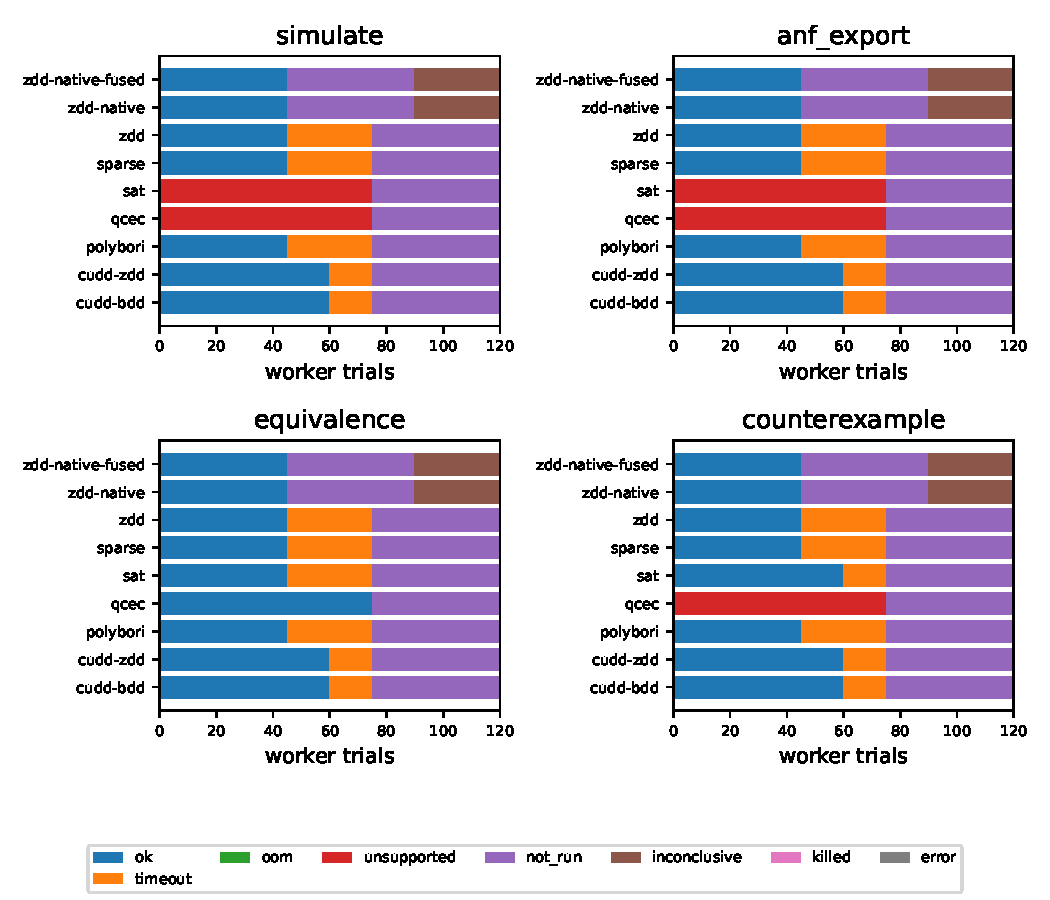
\includegraphics[width=\linewidth]{qualification/coverage.pdf}
\caption{Current public-boundary qualification coverage. Stacks count requested worker trials,
including unsupported/unrun work; repeated trials are not independent programs. Task panels
remain separate. Ratios computed only on common successes cannot establish this coverage.}
\label{fig:current-coverage}
\end{figure}

\begin{figure}[tbp]
\centering
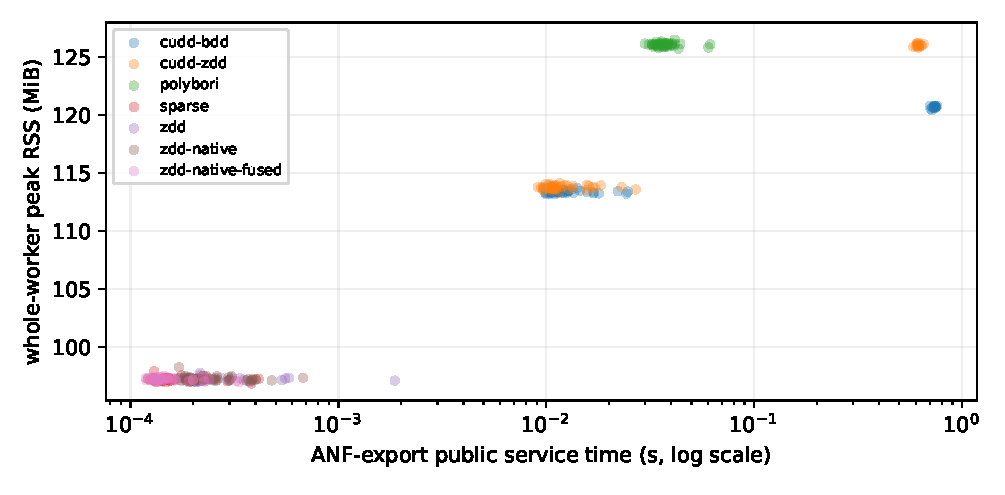
\includegraphics[width=.78\linewidth]{qualification/cost_rss.pdf}
\caption{Current ANF-export service cost and whole-worker peak RSS on successful trials.
Points are descriptive repeats from different families and sizes, not an isolated causal
memory or order ablation. Imports/native heaps contribute to RSS. Failures remain visible in
Table~\ref{tab:current-coverage}; they do not disappear from the scientific denominator.}
\label{fig:current-memory}
\end{figure}

\section{Historical exploration and limits of transfer}\label{sec:historical}
The October 27 campaigns are preserved at their original sources and native binary
\texttt{2e3f6791\ldots}, which predates known count-overflow and width-64 import repairs.
Their figures concern old drivers/cache regimes and cannot be asserted for today's engine.
They found both narrow gains and adverse cases: on the old explored generated corpus the
native minimal loop completed \BNativeLoopOk/\BNativeLoopCells{} requested cells, PolyBoRi
\BPBLoopOk/\BPBLoopCells{}, versus \BBDDLoopOk/\BBDDLoopCells{} for
dynamic CUDD; these are protocol-specific counts with censoring, not equal-budget solved
fractions of independent instances. The old native/PolyBoRi simulation ratio was \BPBSim{} on
\BPBSimN/\BPBSimPairs{} common completed circuits, while the native/dynamic-BDD ratio was
\BBDDSim{} on \BBDDSimN/\BBDDSimPairs{}; its
interval included one. Factor sorting was adverse, whereas fusion helped after correcting
input-construction timing. No one ratio is a statement about current implementation performance.

The old five families had dependent size variants. Binding-cost subtraction was only a
sensitivity analysis on calibrated cache-hit operands, not a bound or proof of causality.
Source replacement during execution, shared-memory kills and repaired/relabelled cells are
listed in \path{paper/REPRODUCIBILITY.md}; full raw and derived sealed files remain intact.
Old tables can be regenerated but are prominently labeled historical. A new campaign does
not erase those negative observations or turn the old holdout back into an unseen one.

\section{Limits, use and release gates}
The measured short corpus qualifies only its cases, interfaces and resource accounting.
It does not establish a broad compiler-workload advantage, machine-independent speed,
optimal variable order, useful support above 128 variables, or a universal ANF strategy.
ANF materialization can be exponential even when a BDD/SAT verdict is cheap. Neither compact
ZDD roots nor a wider mask removes that expansion. Full worker RSS is not live-node memory;
sanitizer timings are not release timings; precompiled kernels are not public calls.
The observed adverse native limit concerns allocated manager nodes, including intermediates
and nodes no longer reachable from final roots. It establishes no lower bound on the final
reachable DAG or ANF size; collection and different orders might alter the frontier, and
their benefit on these particular cases is unmeasured.

The repository also has installed experimental sign/HMR channels, reduced channels,
coherent domains, instruments and bounded dyadic/cyclotomic references. Public Qualtran
fixtures and small Kraus oracles now exist, unlike the historical prototype description.
Those capabilities have their own grammar, input preparation, output observation and
coherence obligations; they are not established by the classical propositions here. The
separate qualification must reject unjustified extensions and may properly recommend
continued experimental status. The separately published public-fixture qualification
recommends precisely that status for its two small Qualtran sizes, rather than promotion
or a large-multiplier claim. Its immutable data revision is
\href{https://github.com/yoch/symq/commit/07f0324c3d9d1cc2df85ea776f22601ccab87679}{\texttt{07f0324c3d9d}};
it is not pooled with the classical timings here. Two isolated executions of one oracle provide process
independence, not algorithmic diversity. Receipts and disk caches are never proof authority.

The useful outcome is an evidence-based choice: request explicit ANFs only when needed,
compare decision engines on decision service, and retain unsupported/resource failures.
Scientific release still requires independent review of the final source, evidence and
claims, plus author confirmation of content, metadata, disclosure and licensing. No arXiv
submission, release, DOI, external scientific publication or main merge is authorized here.

\section*{Artifact identity and reproducibility}
Source commit: \QualCommit.\\
Native SHA-256: \QualNative.\\
Raw qualification SHA-256: \QualRawHash.
\\Published artifact SHA-256: \QualArtifactHash.
\\Case adjudication SHA-256: \QualClassificationHash.

The raw artifact records the manifest, environment, versions, limits, order and individual
trials; \path{paper/qualification/derived.json} records independent table derivation.
\path{paper/REPRODUCIBILITY.md} gives exact rebuild commands and historical distinctions.
The immutable measured source remains its own commit when a later data/paper commit is
created; table regeneration never relabels it. Tests and CI attach to exact content.

\section*{Author metadata and disclosure}
The author name and affiliation above are inherited from the existing draft; this revision
adds no author, affiliation, funding or consent claim. The earlier draft reported AI-assisted
code, experiments and writing, no funding and no competing interests. The author must
reconfirm the final statements before any submission. AI assistance continued during this
maintenance and scientific-review revision.

\bibliographystyle{plain}
\bibliography{references}
\end{document}
